\par L'itération 2 avait pour objectif d'ajouter le type entier. Puis il fallait pourvoir faire une programme, c'est-à-dire des instructions ordonnées avec des étiquettes exécutables plus tard. Pour compléter les objectifs de cette itération certaines commandes et instructions ont été réalisées (efface, liste, lance/affiche, entre, vaen, procedure, stop, retour).

\section{Diagrammes d'objets}
Comme conseillé par notre tuteur, nous avons commencé la conception de l'itération 2 par des diagrammes d'objets. Ci-dessous quelques exemples.
\par
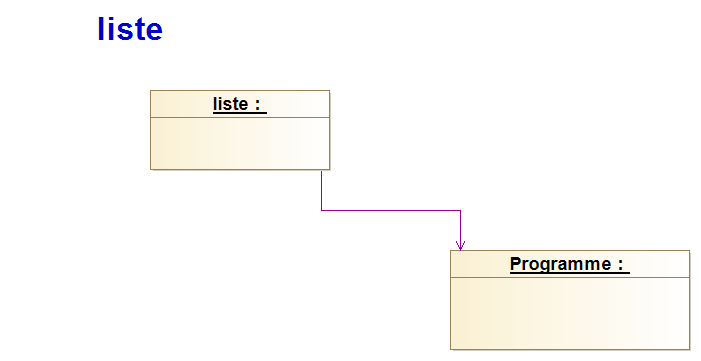
\includegraphics[scale=0.5]{./img/COO/COO_prototype_2/digrammesObjet/Diagramme d'objet la commande liste}
\par Le premier montre que la commande liste fait appel au programme (contenant les lignes de codes constituant un programmes) pour exécuter son comportement.
\par
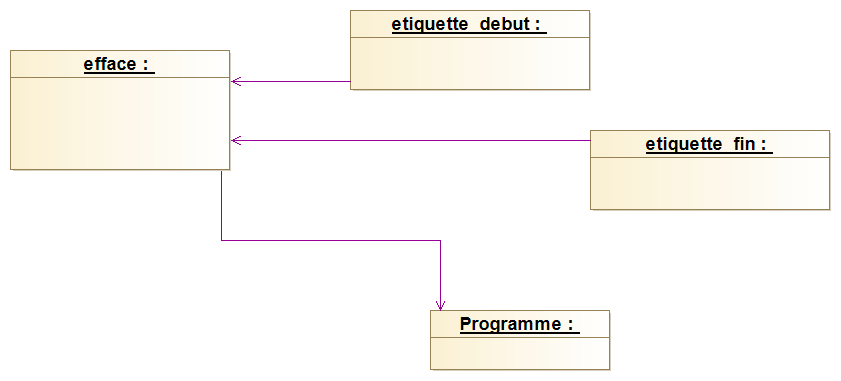
\includegraphics[scale=0.5]{./img/COO/COO_prototype_2/digrammesObjet/Diagramme d'objet de la commande efface}
\par La commande efface connait donc les deux étiquettes qui définissent sont comportement spécifique d'instance. Pour sont exécution elle doit connaitre le programme global de la session courante de l'interpréteur LIR.

\section{Paquetage interpreteurlir.donnees(.litteraux)}
\par Les paquetages donnees et litteraux n'ont que très peu changé en conception mais les classe liées aux entiers ont été codés pendant cette itération.

\section{Paquetage interpreteurlir.expressions}
\par Comme pour les données, pas de changement de conception mais programmtion de ExpressionEntier.

\section{Paquetage interpreteurlir.programmes}
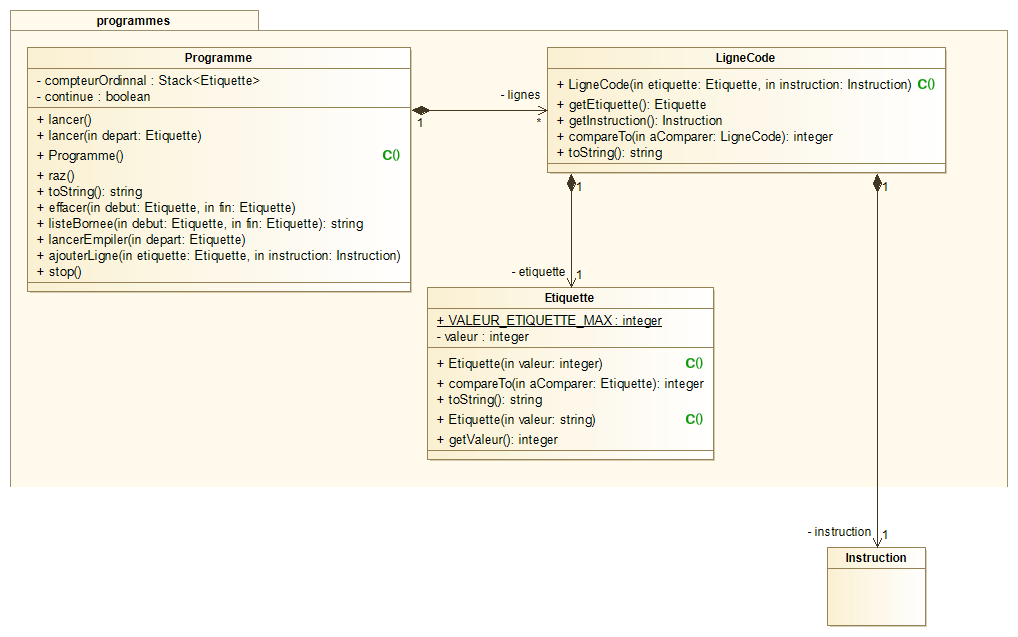
\includegraphics[scale=0.5]{./img/COO/COO_prototype_2/PackageProgrammes}
\par Premièrement la classe étiquette permet d'ordonner les lignes de codes. Le Programme contient des méthodes pour tous les comportement qu'il doit réaliser ce qui permet de les intégrés en interne ce qui rend leur usage plus simple pour les commandes et instructions. Seul la méthode vaen est absente de la conception car nous nous sommes rendu compte qu'elle était nécessaire pendant la programmation. Autre changement, le programme doit enregistrés les lignes de codes. La conception montre une classe LigneCode prévue à cet effet cependant sur le conseil de notre tuteur nous avons utilisé une TreeMap<Etiquette, Instruction> ce qui a rendu LigneCode obsolète. La classe avait été programmée et testée mais nous l'avons supprimée car TreeMap était une meilleur solution.

\section{Paquetage interpreteurlir.motscles} 
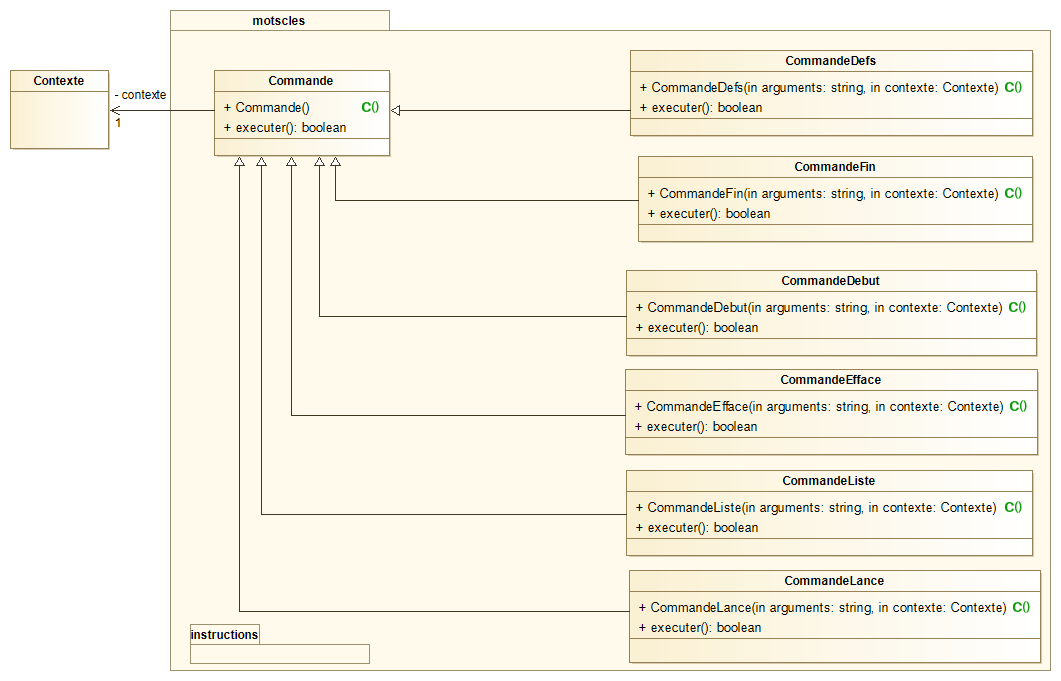
\includegraphics[scale=0.45]{./img/COO/COO_prototype_2/PackageCommande}
\par Les commandes à ajouter à cette itération ont été ajoutée à la conception en suivant le même principe de la dualité construction/exécution. Seul changement notable (non montré dans le diagramme car décidé pendant la programmation), l'ajout du programme nécessite que les commandes connaissent celui-ci. Après une longue réflexion nous avons choisis de le déclaré comme attribut protected dans la classe Commande et de le référencer au lancement de l'interpréteur sans savoir si c'était un bon choix ou non.

\section{Paquetage interpreteurlir.motscles.instructions} 
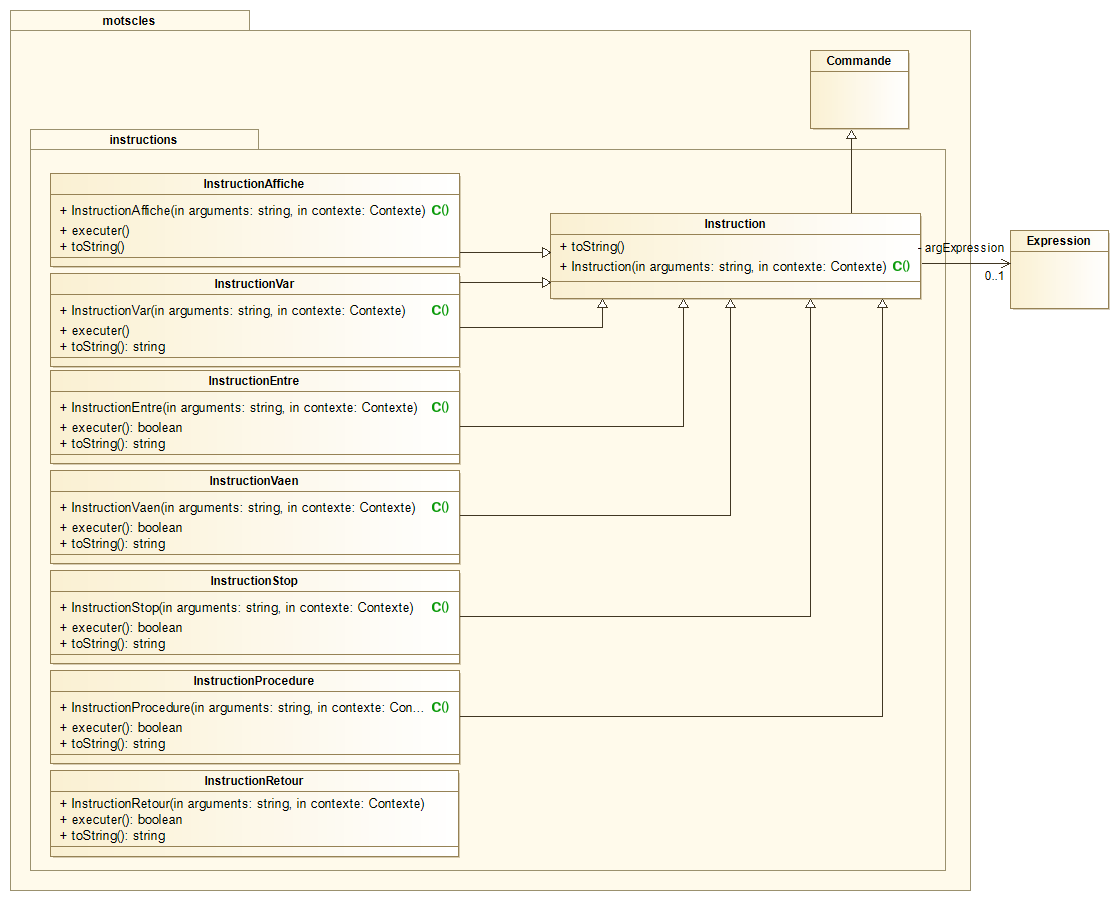
\includegraphics[scale=0.45]{./img/COO/COO_prototype_2/PackageInstruction}
\par Aucun changement notable, seulement ajout des nouvelles instructions.

\section{Paquetage interpreteurlir}
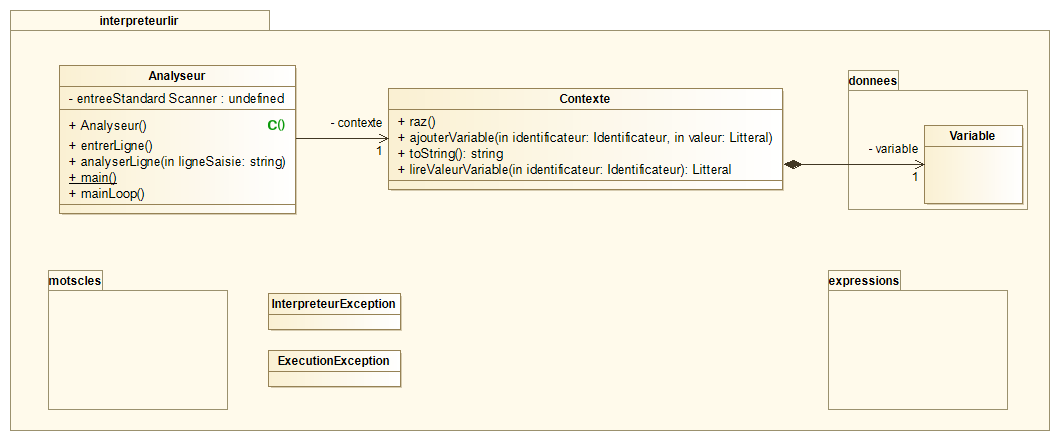
\includegraphics[scale=0.45]{./img/COO/COO_prototype_2/PackageInterpreteurlir}
\par Ajout de l'exception ExecutionException lancée pour une erreur à l'exécution comme une division par 0 (contrairement à l'InterpreteurException qui est lancée à la construction). Elle également affichée par l'Analyseur.